

\section{Overview}
\label{sec:hublink_overview}
% Der HubLink Retriever besitzt eine Indizierungs und Retrieval Phase. In der Indizierungsphase werden die entsprechenden Datenstrukturen vorbereitet, um in der Retrieval Phase die relevanten Informationen zu finden.

% \paragraph{Hubs} Als Hubs werden spezielle Entitäten im Graph klassifiziert, die für eine bestimmte Domäne oder Fragestellung von besonderer Bedeutung sind. Sie bündeln Informationen und bilden so eine Art Dreh- und Angelpunkt für die Suche nach relevanten Informationen. 

% \paragraph{Link} Als Link wird die Verbindung zwischen den Hubs gekennzeichnet, die während dem Retrieval Prozess aufgebaut wird. Dieser Link wird genutzt um die Informationen zwischen den Hubs zu aggregieren und so eine Antwort auf die Fragestellung zu finden.

% Der HubLink Retriever besteht aus insgesamt drei Phasen: der Indexierungsphase, der Retrievalphase und der Antwortgenerierungsphase. In der \emph{Indexierungsphase} werden die Datenstrukturen vorbereitet, um in der Retrievalphase die relevanten Informationen zu finden. In der \emph{Retrievalphase} werden zu der gegebenen Frage die relevanten Hubs  mit Informationen aus dem \gls{kg} gesucht. Zusätzlich werden die Hubs mit externen Informationen verlinkt, um so mehr Kontext zu erhalten. In der \emph{Antwortgenerierungsphase} wird für jeden Hub der als Relevant betrachtet wird, eine Teilantwort generiert. Aus der Menge an Teilantworten wird dann die finale Antwort generiert.In den folgenden Abschnitten werden wir auf die Indexierungsphase genauer eingehen. Anschließend stellen wir zwei verschiedene Strategien vor mit denen der HubLink Retriever arbeiten kann. Beide Strategien beinhalten jeweils die Retrieval- und Antwortgenerierungsphase.

% \begin{figure}[t]
%     \centering
%     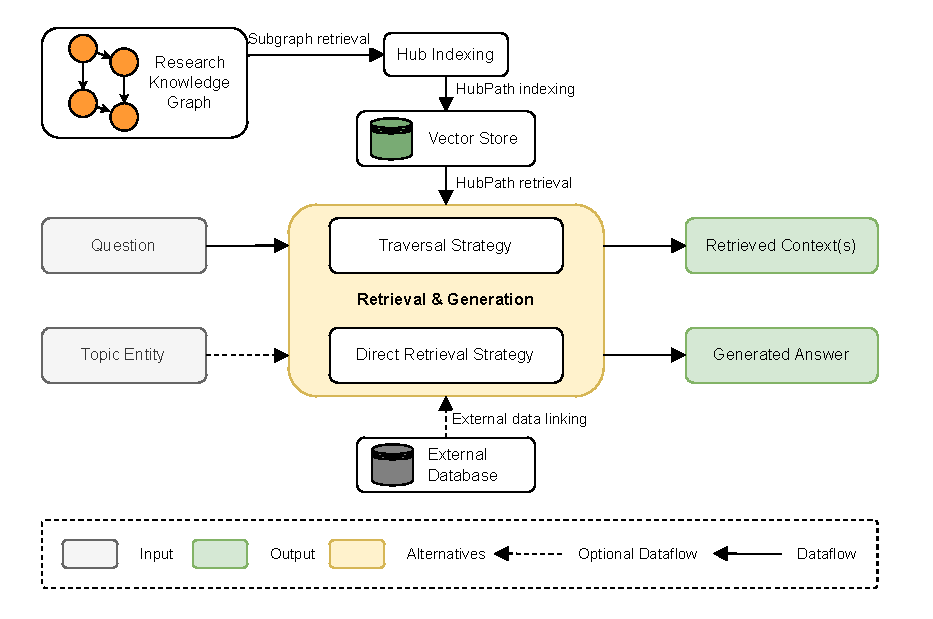
\includegraphics[width=0.95\linewidth]{figures/hublink/Hublink_figures-high_level.drawio.pdf}
%     \caption{High Level Overview of the Dataflow in HubLink}
%     \label{fig:hublink_high_level_overview}
% \end{figure}

% The dataflow of the HubLink retriever is shown in \autoref{fig:hublink_high_level_overview}. The first step of the retriever is the indexing process in which subgraphs are retrieved from an \gls{rkg}. The subgraphs consist of paths which in turn consist of triples. In the HubLink retriever, a subgraph is converted to so called \emph{HubPaths} which are stored in objects referred to as \emph{Hubs}. These are then stored in a vector store in form of low-dimensional vectors. The detailed indexing process is explained in 

This section provides an overview of our proposed HubLink approach. The purpose of this section is to illustrate the overall processes involved before diving deeper into the details in subsequent sections.

HubLink is fundamentally a \gls{grag} technique, which is characterized by its three graph-based stages: indexing, retrieval, and generation. In the following, Section~\ref{sec:hublink_indexing_process_overview} begins with the indexing process, a required preprocessing step that needs to be performed before retrieval to decompose the graph into subgraph structures referred to as \emph{hubs}. After indexing, the retrieval and generation process will be presented in Section~\ref{sec:hublink_overview_retrieval_generation}. Here, the HubLink retriever utilizes one of two different strategies to retrieve relevant data from the index. 

\subsection{Indexing}
\label{sec:hublink_indexing_process_overview}

\begin{figure}[t]
    \centering
    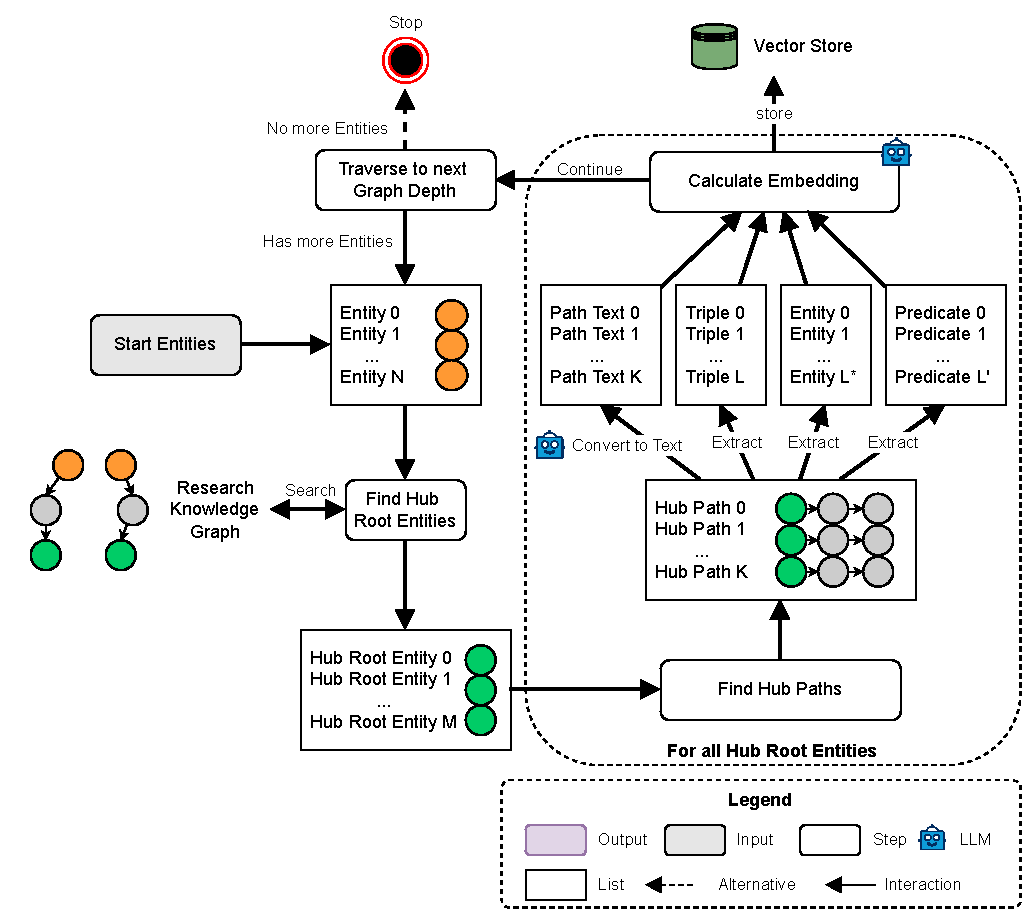
\includegraphics[width=0.93\textwidth]{figures/hublink/Hublink_figures-Overview_indexing.drawio.pdf}
    \caption[Overview of the Indexing Process]{An overview of the indexing process of HubLink showcasing how data is extracted from the \gls{kg} and stored in a vector store.}
    \label{fig:hublink_overview_indexing}
\end{figure}

The indexing process is illustrated in \autoref{fig:hublink_overview_indexing}. It begins with a set of start entities from the graph that serve as initial points for indexing. Using these entities, a search is performed with the goal of finding root entities of hubs. These are specific entities in the graph from which each hub is built. To find these roots, each possible path is traversed until either the end of the graph or until an entity in the graph is reached that is classified as the root of a hub. These identified entities are referred to as \texttt{HubRoot} objects, which are stored in a list to be processed sequentially.

For each identified \texttt{HubRoot} entity, the algorithm continues by finding and building the so-called \texttt{HubPaths}. These paths start from the \texttt{HubRoot} entity and lead to the end entities of a hub, which are either leaf nodes in the graph or other entities classified as roots of a hub. Both \texttt{HubPaths} and \texttt{HubRoot} form a \texttt{Hub} structure, which act as the central elements during retrieval.

Once the \texttt{HubPaths} of a hub are found, each path undergoes further processing before it can be indexed. First, the entire path is passed to an \gls{llm} to create a textual description of the path. In addition, an extraction of the triples, entities, and predicates from the path is performed. These pieces of information, the textual description, the triples, the entities, and the predicates, are then mapped into a low-dimensional vector space using a pre-trained embedding model. After this transformation, these vectors are stored in a vector store, which enables \gls{ann} search for fast access during the later retrieval stage. Furthermore, additional metadata are attached to each vector. This includes the root identifier of the hub for the identification of the hub to which the vector belongs and the description of the path that was generated previously by an \gls{llm}. This metadata is later required for the retrieval phase of the algorithm.

Once these hubs are indexed, the procedure repeats from the nodes in the graph that form the endpoints of each \texttt{HubPath}, provided they have not yet reached a leaf node. The indexing process stops until either the maximum number of traversal levels is reached or no new hubs are found. When the graph is updated, this update needs to be reflected in the index, which we discuss in Section~\ref{sec:updating_the_index}.

\subsection{Retrieval and Generation}
\label{sec:hublink_overview_retrieval_generation}

\begin{figure}
    \centering
    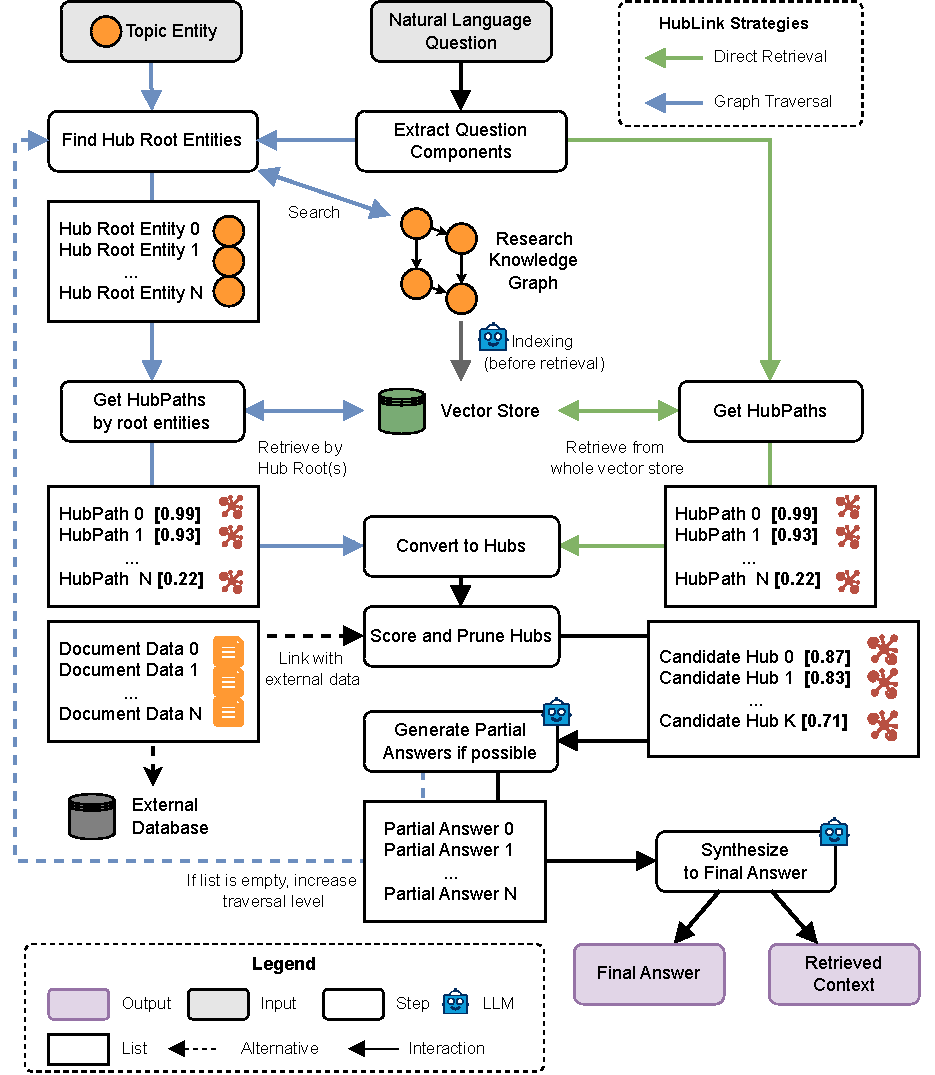
\includegraphics[width=0.98\textwidth]{figures/hublink/Hublink_figures-Overview_topic_strat.drawio.pdf}
    \caption[Overview of the Retrieval and Generation Process]{Overview of the retrieval and generation process: Two alternative strategies are depicted. The process of the direct retrieval strategy is shown with green arrows, while the graph traversal retrieval strategy is highlighted in blue.}
    \label{fig:hublink_retrieval_overview}
\end{figure}

The HubLink retrieval and generation process is illustrated in \autoref{fig:hublink_retrieval_overview}. The retriever offers two strategies for extracting relevant contexts from the \gls{kg}. The first strategy, \emph{Direct Retrieval}, performs a global search on the whole index without requiring access to the graph during retrieval. The second strategy, named \emph{Graph Traversal Retrieval}, performs a subgraph search that begins at a chosen entry point to explore the graph for the identification of relevant hubs to generate answers. The selection of the strategy involves balancing runtime and accuracy, a topic discussed later in this chapter. Both strategies differ only in certain parts of the retrieval algorithm, which we highlight in \autoref{fig:hublink_retrieval_overview} by distinguishing the paths with different colors.

The retrieval begins with an extraction of components from the question. Here, an \gls{llm} is queried to extract the most relevant parts of the question as a list. This list of components and the question itself are then transformed into vectors using the same pre-trained embedding model used in the indexing phase. Now, depending on the strategy applied, the following steps differ:

\paragraph{Graph Traversal Strategy:} In addition to the question itself, this strategy requires as input a point of entry into the graph that is referred to as \emph{Topic Entity}. The algorithm explores all paths starting at the topic entity to find \texttt{HubRoot} entities. After collecting these entities, an \gls{ann} search is performed on the vector store for each collected root entity to find \texttt{HubPaths} that are relevant to the question and contain the root entity in their metadata. This process also involves a deduplication of the paths and the application of a diversity ranker to arrive at the paths that are considered relevant to the question.

\paragraph{Direct Retrieval Strategy:} Unlike the graph traversal strategy, the direct strategy does not require a topic entity for retrieval. Furthermore, during query time, this strategy does not impose any additional queries on the graph itself. Therefore, once the components are extracted from the question, the \gls{ann} search on the vector store is directly started, which involves querying the whole store instead of querying the hubs directly, as done by the traversal strategy. Before the strategy arrives at the final \texttt{HubPaths}, it includes further techniques like clustering by hubs, deduplication of paths, and the application of a diversity ranker. 

The result of both strategies up until this point is a list of hubs with \(n\) \texttt{HubPaths} that the algorithm considers to be the most relevant to answer the question. The next step is to prune the hubs. This is done by aggregating the scores of the paths in each hub by calculating a weighted average. Only the top \(k\) hubs with the highest score are kept for the subsequent steps. 

In the next step, the \emph{Linking} process of the retriever begins. During this process, additional information is searched in an external database using the identifier of the hub, which further enriches the context of the hub beyond the knowledge collected from the graph. This could be, for example, text passages from the source publications.

By now, all necessary information about each hub has been collected. Next, for each hub, a \emph{partial answer} is generated based on the aggregated information from the hub. This is done by passing the information from the hub together with the original question in a prompt to an \gls{llm}. The \gls{llm} first checks if it is possible to provide a partial answer to the question based on this information and then provides the partial answer. If the list of partial answers is empty, no answer could be found for the question. At this step, the traversal strategy continues by traversing deeper into the graph. However, for the direct retrieval strategy, the process ends.

If partial answers have been generated, they are consolidated into a final answer. This is done by passing the partial answers to the \gls{llm} along with the original question. The \gls{llm} then generates the final answer based on this information. 
